\documentclass[letterpaper,oneside,openright,12pt]{book}
\usepackage[spanish]{babel} % Soporte a caracteres de español
\usepackage[utf8]{inputenc} % Acentos directamente en texto
\usepackage{setspace} % Interlineado
\usepackage{verbatim} % Comentarios
\usepackage{pdfpages} % Incluir Paginas de un PDF
\usepackage[shortlabels]{enumitem}
\usepackage{float}
\usepackage{array}

\title{Marco de trabajo para la evaluación de técnicas de visualización de información en los sistemas interactivos}
\author{}
\date{\today}

\setcounter{secnumdepth}{4} % Para enumerar subsubsections
\setcounter{tocdepth}{4} % Para que las subsubsections aparezcan en el indice

\begin{document}
%\includepdf{Portada/Portada}
\maketitle %Portada provicional
\graphicspath{{figures/}}


\newpage
$\ $ % Pagina en Blanco despues de portada
\thispagestyle{empty} 

\doublespacing % Espaciado Doble
\tableofcontents % indice de contenidos
\pagenumbering{Roman}

\cleardoublepage
%\addcontentsline{toc}{chapter}{Lista de figuras} % para que aparezca en el indice de contenidos
%\listoffigures % indice de figuras

\cleardoublepage
%\addcontentsline{toc}{chapter}{Lista de tablas} % para que aparezca en el indice de contenidos
%\listoftables % indice de tablas

\chapter{Introducción}\label{cap.introduccion}
\pagenumbering{arabic} % para empezar la numeración con números
Las pruebas y evaluaciones de usabilidad durante el desarrollo sistemas interactivos han ganado amplia aceptación como estrategia para mejorar la calidad del producto. La introducción temprana de las perspectivas de usabilidad en un producto es muy importante para brindar una clara visibilidad de aspectos de calidad, tanto para los desarrolladores como los usuarios de pruebas. Sin embargo, la evaluación y pruebas de usabilidad no es común que se tomen en cuenta como elementos indispensables del proceso de desarrollo de software\cite{florian2013propuesta} .\\
Con el exponencial avance de las tecnologías que prácticamente han invadido progresivamente todos los aspectos de nuestras vidas. En el trabajo, el estudio o el entretenimiento, nuestras actividades cotidianas cada vez se encuentran más automatizadas, con herramientas y sistemas que intentan mejorar nuestra productividad, comodidad y capacidad de acción. En este devenir tecnológico, computadoras y personas están abocados inevitablemente al entendimiento mutuo.\\
Mientras las nuevas tecnologías tanto en hardware como en software contribuyen a un aumento en el volumen y la diversidad de los datos que las organizaciones manejan, la exploración y la visualización de estos datos se tornan cada vez más dificultosas. Por esto, y debido al crecimiento en la cantidad y variedad de usuarios y a la demanda de mayor funcionalidad, es deseable que los sistemas de Visualización de Información (VI) cumplan con propiedades como la extensibilidad, la modificabilidad, la predictibilidad y la posibilidad de estar integrados por componentes intercambiables \cite{martig2003modelo}. \\
Los sistemas interactivos proporcionan información a través de mecanismos visuales que los usuarios utilizan para comprender lo que sucede en el desarrollo de una actividad individual o colaborativa. La información mostrada a los equipos apoya la generación a la toma de decisiones, comunicación, colaboración y coordinación de los integrantes del equipo\cite{garcia2018factores}.Es por esto qué la Visualización de la Información (VI) es un campo de investigación que ha cobrado gran relevancia en el panorama actual.El término Visualización de la Información fue acuñado a finales de los años 80, y hasta ese momento, es considerado como un sector de la disciplina Interacción Humano-Computadora (IHC).\\
El autor Card define la Visualización de la Información como el uso de soporte informático, interactivo, representaciones visuales de datos abstractos para amplificar la cognición\cite{  card1999readings}. El objetivo de las visualizaciones es transformar una estructura en una gráfica, de manera que esta pueda ser visualizada y el usuario pueda interactuar con ella. Algunas de las técnicas de visualización más conocidas tienen un fuerte componente de interacción que ayuda al usuario a explorar de manera rápida los datos \cite{olmeda2014visualizacion}.\\
A medida que el campo de la visualización de la información aumenta las técnicas desarrolladas en laboratorios de investigación están llegando a los usuarios. Los informes de los estudios de usabilidad y experimentos controlados son útiles, pero hay un deseo creciente de métodos alternativos de evaluación, a fin de presentar evidencia medible de los beneficios para la adopción más generalizada de las técnicas visualización \cite{arjona}.\\
Los marcos de trabajo  pueden ayudar a reducir los costos de desarrollo ya que el objetivo de estos es que posibiliten la evaluación de usabilidad automática.

\section{Definición del problema}
El diseño de técnicas de visualización de información son de carácter genérico, estás se pueden utilizar con una amplia variedad de información y utilizadas en muchos dominios de aplicación. Sin embargo, los usuarios podrían estar insatisfechos si perciben que la técnica de visualización de información no ha sido diseñada específicamente para sus necesidades particulares al caer en errores como que estos no comprenda la técnica de visualización  que se ha elegido  y como consecuencia el usuario  no pueda tomar decisiones de acuerdo con la información que se le está presentando\cite{shneiderman}\\
No se trata solamente de divulgar la información en algun tecnica de visualización, sino de profundizar y aprovechar las ventajas que ofrece la percepción humana y la interacción, con el objetivo de transformar realidades complejas y abstractas en realidades simples.

\section{Preguntas de investigación}
\begin{enumerate}
\item ¿Las evaluaciones de usabilidad son suficientes para evaluar las técnicas de VI?
\item ¿Un marco de trabajo permite la evaluación de técnicas de  VI en los sistemas interactivos?
\end{enumerate}

\section{Objetivos}
\subsection{Objetivo General}
Desarrollar un  marco de trabajo para  evaluar técnicas de VI presentes en los sistemas interactivos
\subsection{Objetivos Específicos}
\begin{enumerate}
\item Seleccionar los criterios que permitan evaluar las técnicas de VI.
\item Diseñar el marco de trabajo con los criterios que permitan evaluar  técnicas de VI para representar el desempeño de equipo.
\item Construir un prototipo con implementación de  técnicas de VI.
\item Evaluar  las técnicas de VI en el prototipo propuesto utilizando el marco de trabajo.
\end{enumerate}

\section{Hipótesis}
La construcción de un marco de trabajo para la evaluación de las técnicas de visualización de información ayuda a la toma de decisión de cuál es la técnica de visualización de información conveniente para utlizar en los sistemas interactivos.

\section{Justificación}
El valor de cualquier sistema de información está condicionado por la calidad y cantidad de información contenida, pero al mismo tiempo por su facilidad para encontrar dicha información, cualidad que naturalmente disminuirá conforme aumente el tamaño del sistema \cite{montero}.
\\Paulatinamente, la visualización científica se fue convirtiendo en uno de los métodos más eficaces para la interpretación de dichos datos, sumando cada vez más fanáticos en la comunidad científica. Gracias a ello y a la evolución de la informática, que nos permite contar con computadoras de bajo costo con gran poderío de cómputo gráfico, los espectros de información se han ampliado, extendiéndose hacia otras disciplinas y para casi cualquier dominio \cite{padua}.
\chapter{Evaluación y técnicas de visualización}\label{cap.Evaluacion}
\pagenumbering{arabic} % para empezar la numeración con números
\section{Evaluaciones de usabilidad}
Evaluar consiste en atribuir un valor a algo o a alguien, en función de un proyecto implícito o explícito. En este sentido, evaluar es una actividad bastante común que realizamos en multitud de ocasiones en nuestra vida cotidiana, y que suele comportar acciones como recoger información, emitir un juicio a partir de una comparación, y tomar una decisión al respecto. La acción de evaluar es algo muy habitual: hay que tomar decisiones constantemente y hay que escoger entre lo que nos conviene y lo que no.\\
Dentro de la disciplina Interacción Humano-Computadora la evaluación de la usabilidad es un proceso para producir una medida de la facilidad de uso. En la evaluación, hay un objeto que está siendo evaluado y un proceso a través del cual uno o más atributos son juzgados o se les da un valor. La evaluación de usabilidad para algunos autores como Mathew, es un estudio empírico con usuarios reales del sistema propuesto, con el propósito de proporcionar retroalimentación en el desarrollo de software durante el ciclo de vida de desarrollo iterativo. El concepto de evaluación de usabilidad es para permitir la validación de todos los requisitos, para hacerlo tan útil como sea posible y así aumentar la calidad del producto y la satisfacción del cliente del producto potencial.\\
La evaluación de la usabilidad, es una de las tareas más importantes que debe emprenderse cuando se desarrolla una interfaz de usuario.Las interfaces pobres pueden, en el ambiente comercial, ahuyentar a clientes potenciales o en el ambiente educativo llevar al fracaso a un aprendiz. En el mundo competitivo de ingeniería de software, una interfaz pobre puede empujar a los usuarios a las manos de la competencia.\\
Algunos métodos de evaluación pueden requerir un completo laboratorio de usabilidad y otros pueden lograrse con poco más que una interacción semi-formal entre el grupo de desarrollo y los usuarios. Incluso con una inversión relativamente pequeña en métodos de usabilidad puede obtenerse una mejora significativa de la usabilidad de un sistema de software \cite{obeso}.
algunas técnicas para la evaluación de usabilidad son: Evaluación heurística, test de usuarios, card sorting y eye tracking.
\subsection{Evaluación heurística}
La evaluación heurística, Es un método de inspección de la usabilidad sin usuarios, propuesta originalmente por Molich y Nielsen (1990). En esta técnica varios expertos inspeccionan y analizan el diseño en busca de potenciales problemas de usabilidad, comprobando para ello el cumplimiento de principios de diseño usable (principios heurísticos) previamente establecidos. Estos principios de diseño o “heurísticas” son directrices que establecen requisitos que debe cumplir el diseño con el fin de facilitar su comprensión y uso por el usuario final.\\
La evaluación heurística se realiza con un ideal de expertos que debe ser entre 3 y 5. Cada uno de los evaluadores examinará el diseño de forma independiente, documentando los problemas de usabilidad detectados. Una vez finalicen su trabajo, harán una puesta en común de los problemas, y se procederá a elaborar un informe final consensuado. Si la evaluación se hace con menos de tres evaluadores, muchos problemas de usabilidad quedarán sin detectar, y usar más de 5 aumentaría el coste de la evaluación sin ofrecer resultados que los justificasen \cite{gonzalez2001evaluacion}.\\
La evaluación heurística, por lo sencillo y económico de su proceso, puede llevarse a cabo en cualquier momento del ciclo de desarrollo del proyecto, un momento idóneo para su realización es antes de estas pruebas con usuarios. Dependiendo del momento de aplicación de la evaluación heurística, los principios o criterios a comprobar podrían variar. En las etapas más tempranas se suelen verificar criterios relacionados con la arquitectura de información, mientras que en etapas posteriores, cuando el diseño se encuentra más elaborado, entrarán en juego también principios de diseño gráfico o visual.\\
Una de las desventajas de la evaluación heurística puede reportar falsas alarmas. Es decir, identificar como un problema de usabilidad aquello que realmente no lo es.
\subsection{Test de usuarios}
El test de usuarios es la prueba reina del diseño centrado en el usuario ya que representa la mejor forma de evaluar la usabilidad de un diseño. Estas pruebas se basan en la observación de cómo un grupo de usuarios llevan a cabo una serie de tareas encomendadas por el evaluador, analizando los problemas de usabilidad con los que se encuentran.\\
Aún cuando el diseñador tenga amplios conocimientos sobre usabilidad, resulta recomendable evaluar el diseño con usuarios. Esto se debe a que, conforme más tiempo dedica un diseñador a un proyecto, menor es su perspectiva y más difícilmente detectará posibles problemas. Podemos decir que gran parte de lo que el diseñador percibe cuando mira su propia obra, es una construcción mental; ve aquello que tiene en mente, no aquello que sus usuarios tendrán ante sus ojos \cite{hassan2003metodo}.\\
Para el test de usuarios el número de participantes que son necesarios para detectar el 100 de los problemas (más importantes) de usabilidad de un diseño se encuentra en torno a 15. Nielsen  recomienda que, en vez de hacer una prueba con 15 participantes, es mejor llevar a cabo tres pruebas con 5 participantes por cada una, repartidas en diferentes momentos del proceso de desarrollo.\\
Esta evaluación debe realizarse en las etapas más tempranas del proyecto, ya que el producto aún no ha tomado forma, los test de usuarios deben realizarse sobre prototipos.\\
El primer problema de los test de usuarios es el alto costo que implica tanto el reclutamiento de los participantes, como el tiempo y esfuerzo dedicados a realizar las pruebas y a sintetizar y analizar los resultados.\\ 
El otro problema es que, al tratarse de pruebas que se realizan en laboratorio y en las que los objetivos y tareas se les imponen explícitamente a los participantes, la interacción del usuario se encuentra descontextualizada, influyendo en su forma de resolver problemas.
\subsection{Card sorting}
Esta técnica consiste en solicitar a un grupo de participantes –que como en el caso del test de usuarios deben tener un perfil acorde con la audiencia a la que se dirige el sitio– que agrupen los conceptos representados en cada tarjeta por su similitud semántica. El objetivo es, por tanto, identificar qué conceptos, de los representados en cada tarjeta, tienen relación semántica entre sí, e incluso cuál es el grado de esa relación.\\ 
 Cómo Lo primero que debemos decidir al planificar una prueba de card sorting es si vamos a realizar un análisis cualitativo de los resultados o uno cuantitativo, ya que esto influirá tanto en el número de participantes como en la forma de dirigir la prueba.\\
En el análisis cualitativo, el número de participantes debe encontrarse en torno de 5. De esta forma podremos acompañar a cada participante en su tarea, e interrogarle acerca de por qué toma la decisión de agrupar unos conceptos u otros y con qué problemas de comprensión se encuentra durante la prueba.\\
Con el análisis cuantitativo, por el contrario, lo que buscamos es una imagen global de las relaciones semánticas entre conceptos. No buscamos tanto un conocimiento en detalle de cómo los usuarios entienden que se relacionan los conceptos, como obtener las relaciones semánticas compartidas y colectivamente más reforzadas que tienen los conceptos para la audiencia del sitio web. En este tipo de análisis, para que los resultados sean representativos, debemos contar con un número mayor de participantes, que Tullis y Wood estiman entre 20 y 30.
El card sorting es una prueba destinada a adaptar la arquitectura de información al modelo mental del usuario, por tanto tiene lugar en etapas tempranas del proyecto (arquitectura de información).\\
Aunque muchos autores coinciden en afirmar que el card sorting es un método rápido, fiable y barato Antolí menciona en que su uso inexperto o inadecuado puede producir resultados erróneos.
\subsection{Eye tracking}
Una de las mayores características del ser humano a diferencia de otra especies es su capacidad para interiorizar y procesar información, transformándola en conocimiento
Desde el punto de vista empírico, existe un tipo de pruebas con usuarios que nos permiten estudiar y analizar su exploración visual, denominadas pruebas de eye-tracking o de “seguimiento visual”. El concepto de eye-tracking hace referencia a un conjunto de tecnologías (hardware y software) que permiten monitorizar y registrar la forma en la que una persona mira una determinada escena o imagen, en concreto en qué áreas fija su atención, durante cuánto tiempo y qué orden sigue en su exploración visual.\\
La mayoría de los sistemas de eye-tracking se basan en el uso de cámaras (eye-trackers) que proyectan rayos infrarrojos hacia uno o los dos ojos del participante, infiriendo la zona de la escena visual que el usuario se encuentra atendiendo en cada momento.
Las pruebas de eye-tracking sólo pueden ofrecer información valiosa sobre diseños gráficos elaborados.\\
Los actuales sistemas de eye-tracking disponibles en el mercado presentan en su mayoría un alto grado de precisión, fruto de la larga evolución que ha experimentado esta tecnología en las últimas décadas. Sin embargo, sigue siendo una tecnología cara, un hecho que impide una mayor difusión en el entorno profesional \cite{hassan2009informe}.
\section{Técnicas de visualización de información}
Se entiende por Visualización de Información la utilización de interfaces interactivas cuya finalidad principal es representar con mínimo desorden visual una serie de datos a un usuario final. Es decir, la Visualización información se caracteriza por ser interrelacionar, transformar datos ¸crudos. En información relevante, buscar la mínima perdida de información en dicha transformación, y dirigirse a usuarios que interactúan, transforman e interpretan esta información \cite{cordoba}.
Algunas técnicas de visualización de información son: gráficas , mapas, tablas.
\subsection{Graficas}
Esquema que representa mediante puntos y líneas las relaciones
entre pares de elementos y que se usa para resolver problemas lógicos, topológicos y de cálculo combinatorio. Dentro de las gráficas encontramos las siguientes:
\begin{figure}[H]
\centering
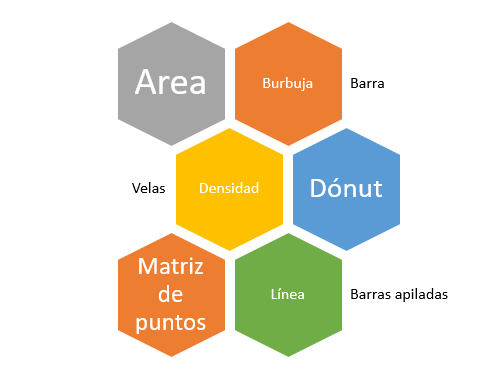
\includegraphics[width=0.7\textwidth]{tipos_graficas.png}
\caption{Tipos de gráficas}
\label{fig:tipos}
\end{figure}

\begin{figure}[H]
\centering

\includegraphics[width=0.7\textwidth]{graficas.jpg}
\caption{Ejemplos de gráficas}
\label{fig:ejemplo}
\end{figure}

\subsection{Mapas}
Representación de conocimiento de manera gráfica \cite{arenas}.
\begin{figure}[H]
\centering
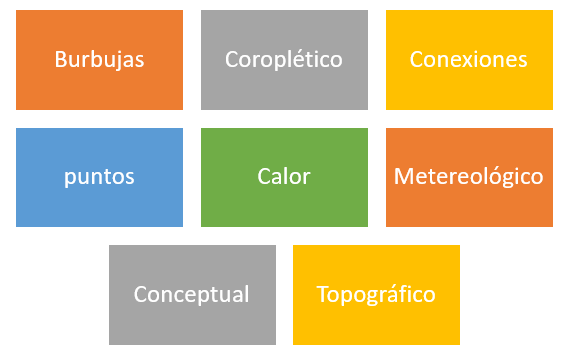
\includegraphics[width=0.7\textwidth]{tipos_mapas.png}
\caption{Tipos de mapas}
\label{fig:tipos}
\end{figure}

\begin{figure}[H]
\centering
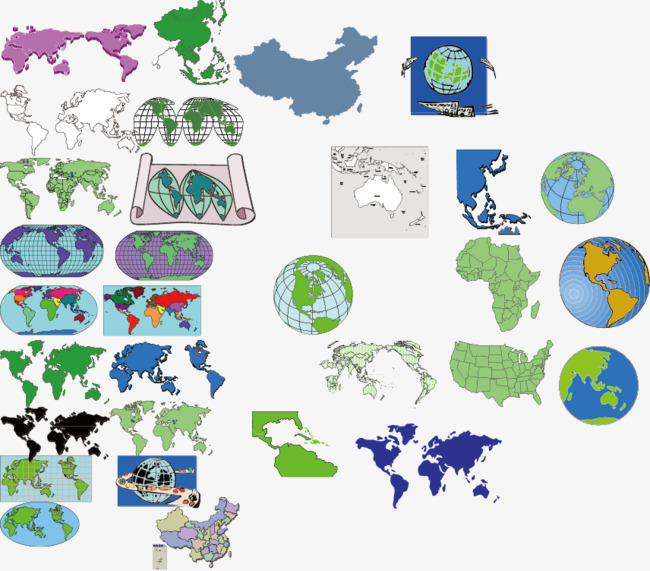
\includegraphics[width=0.7\textwidth]{mapas.jpg}
\caption{Ejemplos de mapas}
\label{fig:ejemplo}
\end{figure}

\subsection{Tablas}
Lista de cosas puestas por orden sucesivo o relacionado entre sí
\begin{figure}[H]
\centering
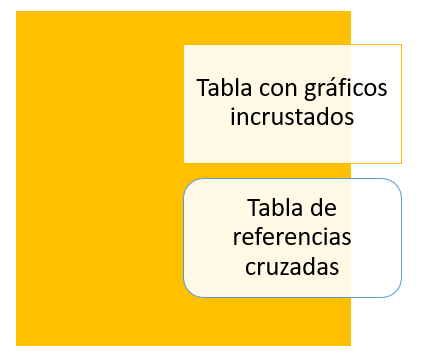
\includegraphics[width=0.7\textwidth]{tipos_tablas.png}
\caption{Tipos de tablas}
\label{fig:tipo}
\end{figure}

\subsection{Principios de diseño}
Los elementos básicos para el diseño de interacción que las técnicas de VI tienen que garantizar son: \\
\begin{enumerate}
\item Visibilidad. Indicadores claros de los datos (color, línea, sombra, dirección, etc.),capaces de manejar numerosos ítems 
\item Retroalimentación. La interfaz gráfica debe soportar todas las tareas de feedback (establecer la coordinación ojo-mano, crear bien definidas metáforas de interacción y permitir un rápido y constante feedback). 
\item Affordances. Mejoran la comunicación entre el usuario y el sistema 
\item Restricciones. El uso de criterios cognitivos mejora el diseño de interacción.
\item Consistencia. Las visualizaciones han de representar y explorar las relaciones entre múltiples estructuras jerárquicas y buscar la afinidad entre la representación y la interfaz gráfica de usuario más estándar (GUI)\cite{arjona}.
\end{enumerate}


%\section{Desempeño de equipos}
%Un equipo es un pequeño número de personas con habilidades complementarias, que están comprometidas con un propósito, un conjunto de metas de desempeño y un enfoque común, por los cuales se hacen mutuamente responsables\cite{katzenbach}.
%El trabajo en equipo que está relacionado con el conocimiento, las habilidades y las actitudes o acciones de los miembros del equipo. Entre los atributos clave para el buen rendimiento de equipos destaca el reconocimiento de la interdependencia y consciencia de equipo, al igual que la identificación de responsabilidades, fortalezas y debilidades de cada integrante.\\
%La medición de desempeño no es algo nuevo y siempre ha estado presente como un mecanismo de verificación y como una importante ayuda para tomar decisiones para llevar acabo la medición de desempeño de equipo se hace necesaria la utilización de un conjuntos de indicadores, en contexto un  indicador se define como una señal que proporciona una información específica acerca de un tema particular, que tiene significado para quien lo utiliza y que cumple un fin específico \cite{arriagada}.\\
%El desempeño se lleva a cabo midiendo el rendimiento de los equipos o enfocada al desempeño individual del usuario dentro del equipo.
%Una medida en particular del desempeño de equipos es el rendimiento del equipo es la Presencia Social, una medida del tipo atomístico para el desempeño de equipo. La presencia social es definida como el grado de relevancia que tienen los usuarios durante una actividad.
%Tambien se tienen algunos otros criterios para medir el desempeño de equipo de manera individual como son las actividades o contribuiciones que realizan.
\subsection{Sistemas interactivos}
Son sistemas que sirven de interconexión entre personas y la computadora y que favorecen la realización de las tareas y el alcance de los objetivos. Donde participan dos actores el usuario y el dispositivo.
\begin{itemize}
\item El usuario: Él interactúa con el sistema para desarrollar una tarea concreta, buscando conseguir objetivos determinados.
\item El Dispositivo: Conjunto de software y hardware específico, para conocer y captar información directamente del entorno.
\end{itemize}
Estos sistemas tienen una interfaz de usuario que funciona como el medio para que el usuario puede comunicarse con un dispositivo\cite{sistemas}.\\
Alguna clasificación de los sistemas interactivos son \cite{raskin2000humane}
\begin{itemize}
\item Sitios web. Es una estructura de información y/o comunicación generada en el nuevo ámbito o espacio de comunicación (Internet), creado por la aplicación de las tecnologías de la información (tecnologías de creación, mantenimiento y desarrollo de los sitios web), que posee dos elementos fundamentales (acciones de los sujetos y contenidos) y en donde se plantean un conjunto de prestaciones que los usuarios que visitan dicho web pueden ejercitar para satisfacer una o varias necesidades que posean \cite{alonso2008sitio}
\item CSCW: Trabajo cooperativo asistido por computadora. Sistemas basados en computadoras que apoyan a grupos de personas que trabajan en una tarea común y que proveen una interfaz para un ambiente compartido\cite{geronimo2002sistemas}
\end{itemize}
%\subsection{Presencia social}
%Grado en el que el medio facilita el conocimiento de la otra persona y las relaciones interpersonales durante la interacción.
%El grado de relevancia de la otra persona en la realización de una interacción, y la importancia de las relaciones interpersonales.
%Una actividad puede ser definida en tres niveles: 1) tareas, 2) objetivos y 3) metas. Las tareas permiten a los usuarios culminar sus objetivos, y el cumplimiento exitoso de estos objetivos permite a los usuarios alcanzar sus metas.\\
%La presencia social calculada a partir del procesamiento de las tareas y objetivos ejecutados por un equipo o un actor en un espacio de actividad. Esta función mide el desempeño del actor, el cual forma parte del equipo, y se encuentra participando dentro de un espacio. Por lo tanto, esta función recibe los parámetros de Actor, Espacio y Tiempo. El Actor es el usuario del cual se requiere obtener la presencia social, Espacio es el lugar donde se encuentra el Actor, y donde la actividad ejecutada concentra las tareas y objetivos culminados, además de otra información relevante en la actividad (roles, familias, etc.). Finalmente, el Tiempo, es un parámetro utilizado para medir hasta un punto determinado de la actividad la presencia social\cite{montane}.
%\subsection{Evaluación individual de desempeño}
%El equipo desarrolla una actividad o presenta un producto de equipo y todos los miembros del equipo reciben la misma evaluación del desempeño, independientemente de la contribución individual.\\
%La medición del desempeño se basa en las actividades o productos realizados individualmente. Cada miembro del grupo recibe entonces una media de estos productos, sin tomar en cuenta la aportación o falta de esta al producto de equipo. \\
%Se obtiene el desempeño de cada miembro del equipo evaluando las contribuciones ponderadas de sus actividades o productos al logro del objetivo común.
\section{Marco de trabajo}
Marco de Trabajo del inglés Framework, se define como "un conjunto de componentes físicos y lógicos estructurados de tal forma que permiten ser reutilizados en el diseño y desarrollo de nuevos sistemas de información".En una estructura de soporte definida en la cual otro proyecto de software puede ser organizado y desarrollado, a partir de una estructura software compuesta de componentes personalizables e intercambiables para el desarrollo de una aplicación. Los marcos de trabajo contienen patrones y buenas prácticas que apoyan el desarrollo de un producto y un proceso con calidad. Lo anterior permite vislumbrar la importancia de adoptar un Marco de Trabajo y cómo su selección debe ser una de las actividades relevantes al inicio de todo proceso de desarrollo software.
Se puede definir a un framework como un armazón, que vendría a ser como una estructura el cual contiene técnicas mediante la utilización de todos los elementos que sean necesarios para beneficio del ser humano\cite{rios}.
Los frameworks de evaluación se pueden definir como macro estrategias utilizadas para organizar el proceso de evaluación. Se pueden incluir varios métodosy herramientas de evaluación en un framework(marco) de evaluación.
A continuación se muestran algunos marcos de trabajo que se han realizado para la evaluación:
\begin{itemize}
\item Un Framework Aspectual para la Evaluación de Usabilidad Automática de Tareas.\\
Este trabajo presenta un framework que permite realizar la evaluación de la usabilidad en aplicaciones de escritorio en el contexto de tareas de usuario. El framework consiste en un conjunto de módulos, aspectos y clases, que interactúan y se relacionan de manera tal de ser altamente reusable y sus requerimientos de especialización (configuración) son mínimos.
\item Un framework para el despliegue y evaluación de procesos.\\
Un marco de trabajo para el despliegue y evaluación de procesos software. Este marco de trabajo se basa en la aplicación de las técnicas de la Ingeniería del Software dirigida por modelos y de la integración de información mediante datos abiertos enlazados. Utilizando las primeras, se consigue la adaptación semiautomática de las herramientas de soporte mediante la transformación sucesiva de modelos, partiendo desde el modelo de procesos.
\item A Framework for Integrating Usability Evaluations Methods: The Mawhiba Web Portal Case Study.\\
Propone la combinación de diferentes métodos de evaluación de usabilidad para obtener mejores resultados a la hora de evaluar.
De esta manera tener una mayor cobertura de problemas de usabilidad y una mejor comprensión de las causas subyacentes de estos problemas, y proporcionar datos complementarios y fundamentar las conclusiones extraídas de las evaluaciones.
\end{itemize}



\section{Antecedentes de la investigación}
Es importante crear técnicas de visualización que maximizan la capacidad humana para percibir y comprender información(indicadores de desempeño de equipo) compleja y dinámica estos no serán eficaces sino se utilizan mecanismos de evaluación donde los usuarios exploren los datos\cite{theron} es por esto que sea hace necesario la evaluación de las técnicas de visualización de información , ya existen algunos trabajos donde se busca realizar este tipo de evaluciones\\
Algunos autores como Freitas, Plaisant, Sheiderman, Oliveira, proponen como técnica para realizar la evaluación a las técnicas de visualización de información un conjunto de criterios de usabilidad o llamadas evaluaciones heurísticas \cite {freitas} , estas evaluaciones se aplican a diferentes técnicas de visualización de información como son: graficas, arboles, mapas diagramas \cite{shneiderman}.\\
Análisis cuantitativo y las gráficas son el campo de estudio y evaluación de Isenberg \cite{isenberg}.\\
Blascheck utiliza métodos de análisis visuales para evaluar los arboles,diagramas y mapas \cite{blascheck}.\\
Entrevistas para evaluar las tablas es el trabajo que realiza el autor Adkins \cite{adkins}, Mazza tambien utiliza este tipo de evaluación pero en su caso lo hace para grupos focales y evaluando graficas \cite{mazza}.\\
En la tabla se hace un resumen de cada de estos artículos con el estudio de las dos variables que nos interesan.
\begin{table}[H]
\centering
\begin{tabular}{p{2cm} p{1cm} p{5cm} p{4cm} p{4cm}}
\hline
Autor & Año  & Técnica de evaluación & Técnica de VI \\
\hline \hline
Freitas & 2002 & criterios de usabilidad& Visualización jerárquica  \\
\hline
Isenberg & 2008  & Análisis cuantitativo & Graficas  \\
\hline
Shneiderman & 2006 & Heurísticas de usabilidad  & Diagramas de árbol  \\
\hline
Plaisant & 2004 & Heurísticas de usabilidad & Arboles  \\
\hline
Blascheck & 2013 & Métodos de análisis visuales & Arboles,diagra y mapas  \\
\hline
de Oliveira & 2017 & Heurísticas de usabilidad & Mapas  \\
\hline
Adkins & 2016 & Entrevistas & Tablas  \\
\hline
Mazza & 2007 & Entrevistas en grupos focales & Graficas  \\
\hline
\end{tabular}
\caption{Antecedentes de la investigación}
\label{tabla:autores}
\end{table}
Como parte de la investigación también se busca saber que se ha realizado en cuanto a evaluaciones de tecnicas de visualización de información donde los datos que se representan sea para un grupo de personas y todos ellos esten involucrados en el analisis de la información o a tomar decisiones respecto a la información representada esto en un contexto de equipos de donde se obtienen los siguientes resultados:
Bresciani en su artículo los beneficios de la visualización sincrónica de información colaborativa: evidencia de una evaluación experimental utilizando para la evaluación el método empírico en el contexto del  sector empresarial este autor busca con su trabajo mostrar la relevancia y beneficios de la visualización de información en el contexto de deliberación grupal colaborativa en grupos de gerentes para saber si esta visualización colaborativa ayuda a que haya mayor productividad, aprendizaje, satisfacción y  participación de los gerentes involucrados\cite{bresciani2009benefits}.\\
Otros autores como Isenberg pioneros en la visualización colaborativa en uno de los siete escenarios  estudia la visualización colaborativa para todo un análisis colaborativo de datos y llegar a una conclusión o descubrimiento en conjunto, la evaluación que utilizan es la evaluación heurística, estos autores marcan la importancia de una visualización colaborativa que es apoyar en las tareas y las acciones para el equipo. Uno de los atributos que resaltan en este articulo es que el autor utiliza la eficacia del equipo como una medición para saber si realmente está funcionando la visualización colaborativa \cite{lam2011empirical}.\\
En las redes sociales hay un uso creciente de los sistemas colaborativos los diseñadores los están usando para conectar a grupos pequeños y así poder obtener la interacción colaborativa Mcdonald propone como método de evaluación entrevistas comparando dos redes sociales y así de manera visual podernos dar cuenta como están construidas\cite{ mcdonald2003recommending}.\\
WINKLER decide hacer su evaluación en visualización en 3D ya que afirma que de esta manera las personas pueden ser mas intuitivas a la hora de tomar decisiones utiliza el método empírico para realizar esta evaluación lo que el hace es una representación de imágenes para un grupo de personas ubicados en el mismo lugar y estas imágenes utilizan diferentes vistas de visualización. El espacio de trabajo colaborativo, que incluye múltiples vistas de roles específicos coordinadas con una vista de equipo, permite una clara separación entre datos de roles específicos y compartidos, permite al equipo filtrar detalles específicos de roles y compartir conocimientos estratégicos y permite un aprendizaje fortuito sobre conocimientos y experiencia dentro del equipo\cite{ winkler2008collaborative}.

\begin{table}[H]
\centering
\begin{tabular}{p{2cm} p{1cm} p{5cm} p{4cm} p{4cm}}
\hline
Autor & Año  & Técnica de evaluación & Caso de estudio \\
\hline \hline
Bresciani & 2009 & Método empírico & Empresas  \\
\hline
Isenberg & 2012  & Heurísticas de evaluación & Escenarios \\
\hline
McDonald & 2003 & Entrevistas  & Redes sociales  \\
\hline
Winkler  & 2008 & Método empírico  & Pantallas 3 D  \\
\hline
\end{tabular}
\caption{Trabajos relacionados}
\label{tabla:autores}
\end{table}
 


\chapter{Propuesta}\label{cap.Propuesta}
\pagenumbering{arabic} % para empezar la numeración con números
Después de una revisión de información se pudo notar que estos tipos de evaluaciones de manera individual presentan diferentes problemas ya que algunas al tratarse de pruebas que se realizan en laboratorio y en las que los objetivos y tareas se les imponen explícitamente a los participantes, la interacción del usuario se encuentra descontextualizada, influyendo en su forma de resolver problemas.\\
En la evaluación heurística se permite identificar una mayor cantidad de problemas de usabilidad menores, pero una menor cantidad de problemas de usabilidad mayores que otras metodologías como los test de usuarios. Esto significa que esta metodología no puede sustituir a la realización de test de usuarios, ya que resulta menos eficaz en la detección de aquellos problemas de usabilidad que mayor impacto tendrán en el usuario final.\\
Para el card sorting autores coinciden en afirmar que es un método rápido, fiable y barato en que su uso inexperto o inadecuado puede producir resultados erróneos.\\
En el eye tracking el problema es que, aunque el proceso de calibración visual de los participantes previo a la prueba es rápido y sencillo, existe un significativo porcentaje de personas cuyos ojos no pueden calibrarse, lo que encarece aún más este tipo de estudios.\\
Los trabajos que han consistido en evaluar las técnicas de visualización hacen uso de estos métodos de evaluación tablas 2.2 y 2.2 , sin embargo estas evaluaciones presentan ciertos problemas que anteriormente se mencionaron, en este trabajo se propone un marco de trabajo donde estén implicadas más de un tipo de evaluación para un contexto de visualización de información donde esta información será para mostrar el desempeño que este teniendo un usuario dentro de un equipo.


\bibliographystyle{apalike}
\addcontentsline{toc}{chapter}{Bibliografía}
\bibliography{bibliografia}

\end{document}